% ----------
% A LaTeX template for course project reports
% ----------
\documentclass[12pt, letterpaper, twoside]{article}
\usepackage{geometry}
\usepackage[utf8]{inputenc}
\usepackage[english]{babel}
\usepackage[runin]{abstract}
\usepackage{titling}
\usepackage{booktabs}
\usepackage{fancyhdr}
\usepackage{helvet}
\usepackage{csquotes}
\usepackage{graphicx}
\usepackage{blindtext}
\usepackage{parskip}
\usepackage{etoolbox}
\usepackage{amsmath}

\input{preamble.tex}

% ----------
% Variables
% ----------

\title{\textbf{Simulation and Modeling Course Project:\\Traffic Intersection Simulation}} % Full title of your tech report
\author{Harsh Panchal (100820984)}
\date{\today}

% ----------
% actual document
% ----------
\begin{document}

\begin{center}
    {\Large \textbf{Simulation and Modeling Course Project:\\Traffic Intersection Simulation}}\\
    \vspace{0.5cm}
    \textbf{by}\\
    \vspace{0.5cm}
    Harsh Panchal (100820984)\\
    \vspace{1cm}
\end{center}

\begin{abstract}
    \noindent
    This project investigates the optimization of a 4-way traffic intersection using a 2D hybrid continuous/discrete simulation. The focus is on analyzing how different traffic light cycle lengths and varying vehicle arrival rates impact overall intersection efficiency, specifically targeting the minimization of queue lengths and average wait times, while maximizing throughput. A custom Python physics engine was built to model vehicle kinematics, stochastic spawning, and collision avoidance.
\end{abstract}

\vspace{1.5cm}

\textbf{Repository:}\\
https://github.com/HarshPanchal01/Traffic-Intersection-Simulation

\textbf{Execution:}\\
Run \texttt{python3 main.py} while inside the parent directory using a Python 3.x environment to view the visual simulation.\\
Run \texttt{python3 main.py --headless} to run high-speed batch experiments and generate data plots.

\thispagestyle{firstpage}
\pagebreak

% ----------
% End of first page
% ----------

\newgeometry{} % Redefine geometries (normal margins)

\section{Introduction}
\label{sec:intro}
The primary objective of this project is to simulate a 4-way traffic intersection to evaluate the parameters required to maintain optimal traffic flow. Traffic intersections represent complex systems where continuous physical movements (vehicle kinematics) intersect with discrete events (traffic signal state changes and stochastic vehicle arrivals). 

By developing this simulation, the goal was to study how these systems reach equilibrium and observe their behavior when pushed beyond their carrying capacity. The primary outcomes considered in this study were:
\begin{enumerate}
    \item The impact of varying green light phase durations on the average wait time, queue length, and throughput of vehicles. This seeks to identify an optimal signal timing that minimizes delays.
    \item The system's response to increasing volumes of traffic (arrival rates). This aims to determine the intersection's maximum throughput capacity and the point at which queue lengths grow uncontrollably, indicating systemic failure.
\end{enumerate}

To address these inquiries, the simulation tracks each vehicle's speed, wait time, and position, aggregating this data to evaluate the overall efficiency of the intersection under various configurations.

\section{Inspirations and Related Work}
\label{sec:related}
This project integrates multiple simulation paradigms discussed in the CSCI 3010U Simulation and Modeling course into a cohesive model:
\begin{itemize}
    \item \textbf{Continuous Systems:} The foundational kinematics of the vehicles (acceleration, velocity, position) were inspired by continuous system models (e.g., projectile and mass-spring systems). Ordinary Differential Equations (ODEs) are utilized to govern vehicle movement over time.
    \item \textbf{Discrete Event Systems (DES):} The traffic light state machine and the queueing behavior of vehicles waiting at red lights reflect DES concepts. The intersection acts as a server processing entities (vehicles) from queues.
    \item \textbf{Random Processes:} The generation of traffic is modeled as a Poisson process using inverse transform sampling. This technique mimics natural, unpredictable occurrences, similar to radioactive decay, allowing for realistic, randomized vehicle arrivals.
    \item \textbf{Collision Detection:} The logic required to prevent vehicular collisions within the intersection utilizes distance-based collision detection and spatial awareness techniques.
\end{itemize}

\section{Methodology}
\label{sec:method}
The simulation is implemented in Python, utilizing Pygame for visualization and SciPy/NumPy for mathematical computations. It operates as a hybrid model combining continuous physics and discrete stochastic events.

\subsection{Continuous Kinematics}
Vehicle movement is modeled using a system of first-order ordinary differential equations (ODEs). The state of a vehicle is defined as $\mathbf{s} = [x, v]$, where $x$ is the 1D position along its trajectory and $v$ is its velocity. The derivatives are defined by standard Newtonian kinematics \cite{halliday2013fundamentals} as:
\begin{equation}
    \frac{dx}{dt} = v, \quad \frac{dv}{dt} = a
\end{equation}
where $a$ is the acceleration applied by the driver's behavioral logic. To ensure high physical accuracy and prevent numerical instability during deceleration, the explicit Runge-Kutta 8th order (\texttt{dop853}) solver from SciPy was employed to integrate these equations.

When approaching a red light or a slower vehicle, the driver calculates a safe braking distance using standard kinematic equations, derived from the work-energy theorem \cite{halliday2013fundamentals}:
\begin{equation}
    s = \frac{v_{initial}^2}{2 \times a_{braking}}
\end{equation}
If the distance to the obstacle falls within this braking threshold plus a defined safety buffer, the vehicle applies maximum deceleration.

\subsection{Stochastic Spawning}
To simulate natural traffic flow, vehicles arrive according to a Poisson distribution rather than at fixed intervals. The Inverse Transform Sampling method generates exponentially distributed time gaps between arrivals. Given a desired average arrival rate $\lambda$ (vehicles per second) and a uniform random variable $U \in [0, 1)$, the time $t$ until the next vehicle spawns is calculated using the inverse cumulative distribution function of the exponential distribution \cite{ross2012simulation}:
\begin{equation}
    t = -\frac{1}{\lambda} \ln(1 - U)
\end{equation}
This approach accurately recreates the clustering effect observed in real-world traffic patterns.

\subsection{Collision Avoidance and Intersection Logic}
To address issues with vehicles intersecting during turns, curved paths were unrolled into 1D trajectories. The distance to the preceding vehicle is calculated as the difference in their 1D parametric $x$ states along the mathematical arc.

Additionally, a cross-traffic blocking algorithm prevents gridlock. Before entering the intersection on a green light, a vehicle evaluates the 2D bounding box of the intersection. If opposing traffic is moving below a critical threshold ($< 15$ px/s), the vehicle yields at the stop line, simulating real-world traffic regulations.

\section{Results}
\label{sec:results}
Data was gathered by running the simulation in a headless mode to ensure statistically significant results without rendering overhead. Two primary experiments were conducted, evaluating the system across 5-minute simulated intervals.

\subsection{Experiment 1: Varying Green Light Duration}
In the first experiment, the arrival rate was fixed at 0.5 vehicles/second, and the green light duration was varied from 5 to 60 seconds.

\begin{figure}[h]
    \centering
    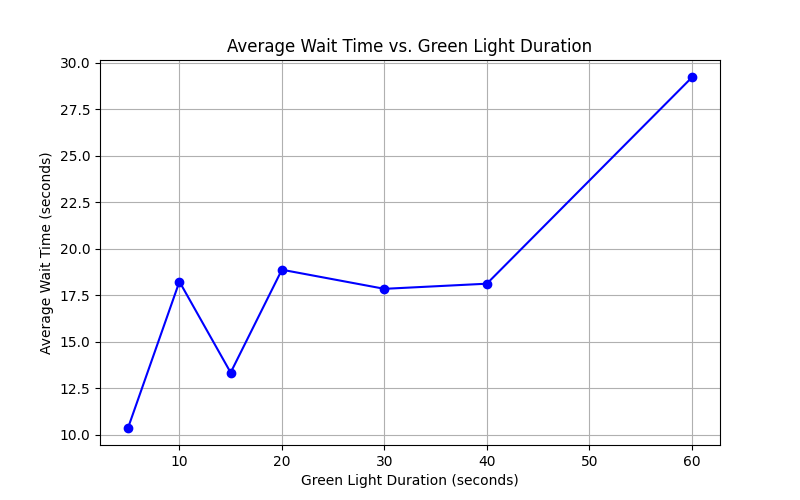
\includegraphics[width=0.7\textwidth]{../analytics/plots/plt_exp1_wait_time.png}
    \caption{Average Wait Time vs. Green Light Duration}
\end{figure}

The data indicates that very short green lights (5s) result in the lowest average wait time (approximately 10 seconds) for this specific traffic volume. As the green light duration extends, wait times generally increase, peaking at nearly 30 seconds when the duration is set to 60 seconds. This occurs because prolonged green phases force cross-traffic to idle excessively, negatively impacting the global average.

\begin{figure}[h]
    \centering
    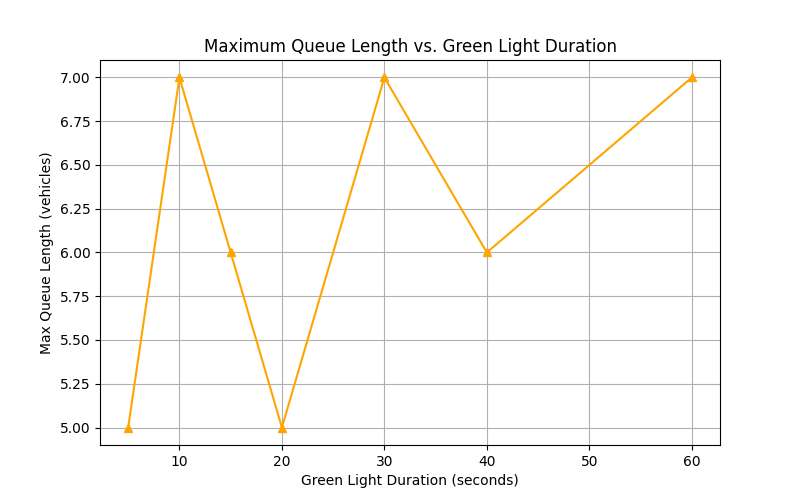
\includegraphics[width=0.7\textwidth]{../analytics/plots/plt_exp1_queue_length.png}
    \caption{Maximum Queue Length vs. Green Light Duration}
\end{figure}

The queue length data shows volatility, with maximum queues fluctuating between 5 and 7 vehicles across different durations. This suggests that while shorter cycles might reduce average wait times, they can occasionally cause rapid localized queuing if a cluster of vehicles arrives during a red phase.

\begin{figure}[h]
    \centering
    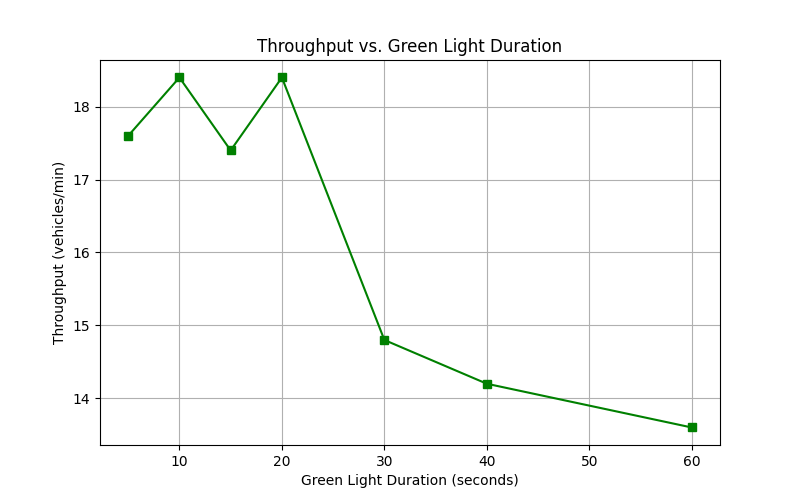
\includegraphics[width=0.7\textwidth]{../analytics/plots/plt_exp1_throughput.png}
    \caption{Throughput vs. Green Light Duration}
\end{figure}

Throughput analysis reveals an optimal performance range between 10 and 20 seconds, achieving roughly 18.5 vehicles/minute. Durations extending beyond 20 seconds show a marked decline in throughput, dropping to approximately 13.6 vehicles/minute at a 60-second duration. This confirms that excessively long cycles introduce inefficiencies that reduce the intersection's overall processing capacity.

\subsection{Experiment 2: Varying Arrival Rate}
In the second experiment, the green light duration was locked at 20 seconds while the traffic volume was increased from 0.1 to 1.25 vehicles/second.

\begin{figure}[h]
    \centering
    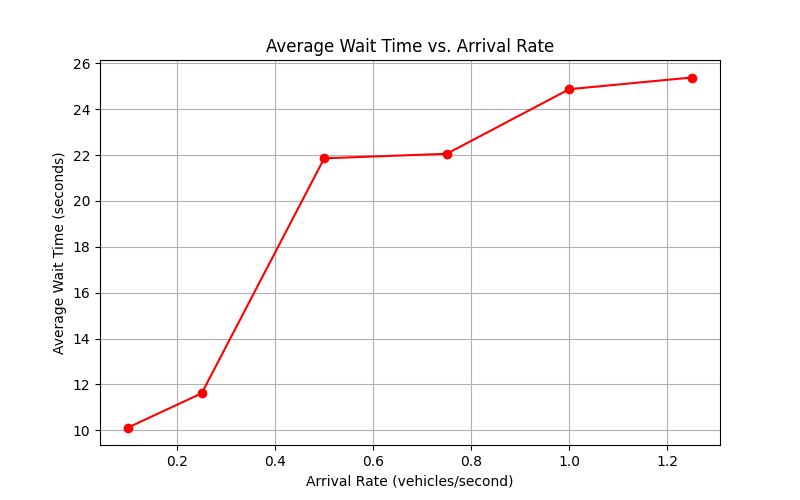
\includegraphics[width=0.7\textwidth]{../analytics/plots/plt_exp2_wait_time.png}
    \caption{Average Wait Time vs. Arrival Rate}
\end{figure}

Average wait times demonstrate a clear inflection point. At lower arrival rates (0.1 to 0.25 v/s), wait times remain stable around 10-11 seconds. However, as the rate approaches 0.5 v/s, the wait time doubles to approximately 22 seconds, indicating the onset of congestion as the system struggles to clear queues within a single cycle.

\begin{figure}[h]
    \centering
    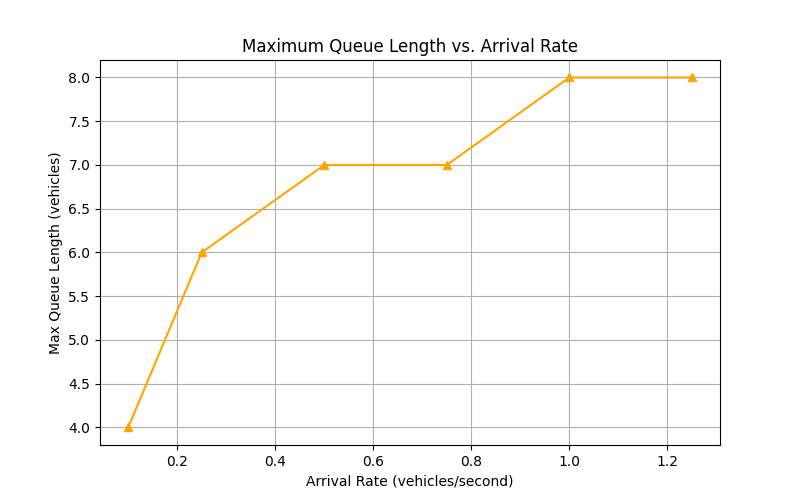
\includegraphics[width=0.7\textwidth]{../analytics/plots/plt_exp2_queue_length.png}
    \caption{Maximum Queue Length vs. Arrival Rate}
\end{figure}

Maximum queue lengths grow proportionally with the arrival rate, rising from 4 vehicles at 0.1 v/s to a plateau of 8 vehicles at rates of 1.0 v/s and above. This plateau suggests that the physical space or the cycle capacity is fully saturated.

\begin{figure}[h]
    \centering
    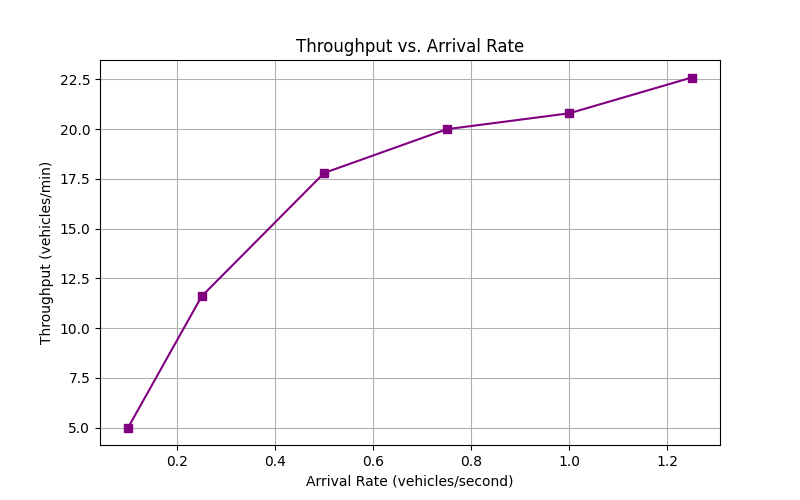
\includegraphics[width=0.7\textwidth]{../analytics/plots/plt_exp2_throughput.png}
    \caption{Throughput vs. Arrival Rate}
\end{figure}

The throughput data clearly illustrates the system's carrying capacity. Throughput climbs linearly alongside the arrival rate initially. However, beyond 0.75 vehicles/second, the growth decelerates, forming an asymptotic ceiling at approximately 22.5 vehicles per minute. At this saturation point, the kinematic limits of vehicle acceleration and mandatory safety distances prevent the intersection from processing additional volume, resulting in unbounded queue growth in a real-world scenario.

\section{Scope and Limitations}
\label{sec:scope}
Several assumptions were made to simplify the simulation model:
\begin{itemize}
    \item Vehicles are assumed to have uniform acceleration and braking capabilities, ignoring the variability present in human drivers and different vehicle classes.
    \item The model operates in a 2D space where lane-changing and complex intersection maneuvers (e.g., dedicated advanced turning lanes) are not fully realized.
    \item The simulation does not account for pedestrian traffic or environmental factors such as weather, which would practically influence driving speeds and reaction times.
\end{itemize}

\section{Discussion and Conclusions}
\label{sec:conc}
This simulation successfully models the complex dynamics of a 4-way traffic intersection. By implementing continuous kinematic bodies and mathematically rigorous Poisson spawners, the model provides realistic insights into traffic waves and congestion thresholds.

The experimental results empirically demonstrate that signal timing must be carefully optimized against traffic volume. Short to moderate cycle lengths (10-20 seconds) maximize throughput and minimize wait times under moderate loads. Furthermore, the system exhibits a definitive physical carrying capacity (approximately 22 vehicles/minute), beyond which increased arrival rates lead to exponential delays and saturated queues. These findings validate the theoretical concepts of discrete event systems and continuous modeling applied to infrastructural analysis.

\section{References}
\label{sec:ref}
\begin{thebibliography}{9}

\bibitem{qureshi2024}
Qureshi, F. Z. (2024). \textit{Simulation and Modeling (CSCI 3010U) Lecture Notes}. Ontario Tech University.

\bibitem{halliday2013fundamentals}
Halliday, D., Resnick, R., \& Walker, J. (2013). \textit{Fundamentals of Physics} (10th ed.). John Wiley \& Sons.

\bibitem{ross2012simulation}
Ross, S. M. (2012). \textit{Simulation} (5th ed.). Academic Press.

\end{thebibliography}

\end{document}